
In this section, we describe our empirical evaluation of the EAGER
prototype and evaluate its overhead and scaling characterists.
We start by presenting the time required for AppScale application deployment
without EAGER as it is this process on which we piggyback EAGER support.  
These measurements are conservative in that they are taken 
from a single VM deployment of AppScale (it is designed to run at scale) so that
logging and timing information is easier to gather.  AppScale uses an
Ubuntu 12.04 Linux image which we hosted using Vagrant~\cite{vagrant}    
on a $2.7$ GHz x86 CPU with $4$ GB of memory.
Table~\ref{tab:sample_apps} lists a number of App Engine
applications that we consider, their artifact size, and their average deployment times 
across three runs, on AppScale without EAGER.
We also identify the number of APIs and dependencies for each 
application in the \texttt{Description} column.
These applications represent a wide range of programming languages,
application sizes, and business domains.  

\begin{table}[t]
\begin{center}
\begin{tabular}{| p{1.5cm} | p{3.2cm} | p{0.5cm} | p{1.1cm} | }
\hline
Application & Description & Size (MB) & Deployment Time (s) \\ \hline
guestbook-py & A simple Python web application that allows users to post
comments and view them & 0.16 & 22.13 \\ \hline
guestbook-java & A Java clone of the guestbook-python app & 52 & 24.18 \\ \hline
appinventor & A popular open source web application that enables creating mobile apps & 198 & 111.47 \\ \hline
coursebuilder & A popular open source web application used to facilitate teaching online courses & 37 & 23.75 \\ \hline
hawkeye & A sample Java application used to test AppScale & 35 & 23.37 \\ \hline
simple-jaxrs-app & A sample JAXRS app that exports 2 web APIs & 34 & 23.45 \\ \hline
dep-jaxrs-app & A sample JAXRS app that exports a web API and has one dependency & 34 & 23.72 \\ \hline
dep-jaxrs-app-v2 & A sample JAXRS app that exports 2 web APIs and has one dependency & 34 & 23.95 \\ \hline
\end{tabular}
\end{center}
\caption{Sample AppScale Applications}
\label{tab:sample_apps}
\end{table}

On average, deployment without EAGER takes $34.5$ seconds and this time 
is correlated with application artifact size.  The total time consists
of network transfer time of the application to the cloud (which is this 
case is via localhost networking) and disk copy to the application servers.
For actual deployments, both components are likely to increase due to network
latency, available bandwidth, contention, and large numbers of distributed
application servers.


\begin{figure}
\centering
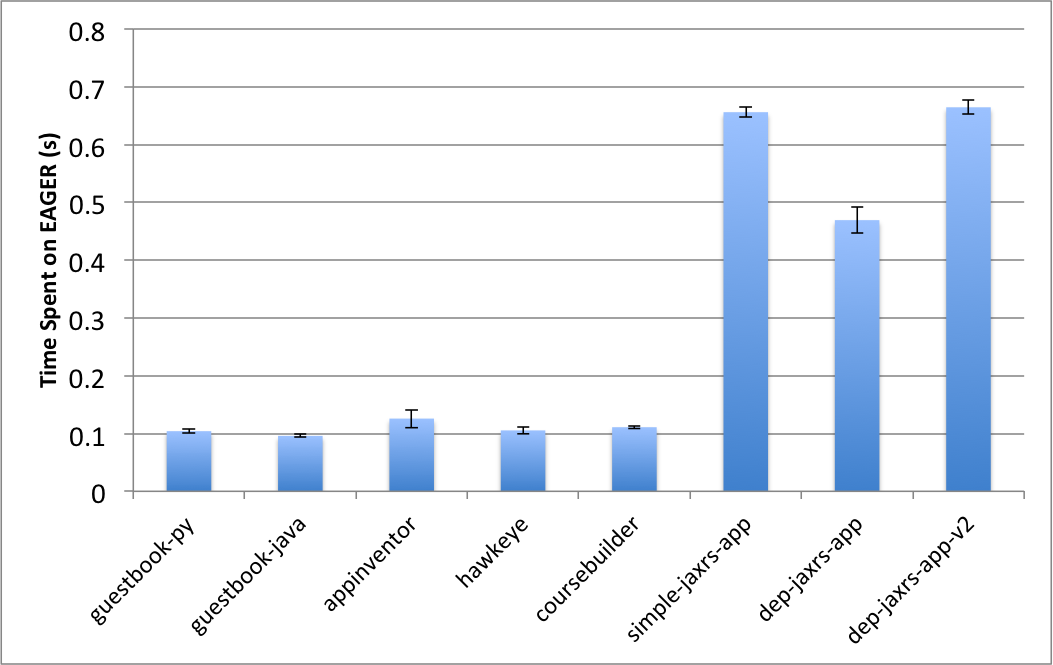
\includegraphics[scale=0.45]{overhead_by_app}
\vspace{-0.01in}
\caption{EAGER Absolute Overhead in Seconds by Application}
\label{fig:overhead_by_app}
\end{figure}

\subsection{Baseline EAGER Overhead by Application}

Figure~\ref{fig:overhead_by_app} shows the time in seconds taken by EAGER to validate and 
verify each application.  We record these results on an EAGER deployment without any policies 
deployed, and without any prior metadata recorded in the API metadata manager 
(that is, an unpopulated database of policies).
We present the values as absolute measurements (here and henceforth) because
of the signficant (order of magnitude) difference between them and 
AppScale deployment time.  We can alternatively observe this overhead as a 
percentage AppScale deployment time by dividing these times by 
those shown in Table~\ref{tab:sample_apps}.


Note that some applications do not export any web APIs;
for these EAGER overhead is negligibly small (approximately $0.1$s). 
This result indicates that EAGER does not impact deployment time of applications 
that do not require API governance.  For applications that do
export web APIs, the recorded overhead measurements include the time
retrieve old API specifications from the Metadata Manager, the time 
to compare the new API specifications with the old ones, the time
update the API specifications and other metadata in the Metadata Manager, and
the time to publish the updated APIs to the cloud.  
The worst case observed overhead for governed APIs (simple-jaxrs-app in the
Figure~\ref{fig:overhead_by_app}) is 2.8\%.


\subsection{Impact of Number of APIs and Dependencies}

Figure~\ref{fig:overhead_by_apis} shows that EAGER overhead grows linearly
with the number of APIs exported by an application.  This scaling occurs
because the current prototype implementation iterates through the APIs in the
application sequentially and records the API metadata in the Metadata Manager.
Then EAGER publishes each API to the ADP and API Gateway. This sequencing
individual EAGER events, each of which generates a separate web service call,
represents an optimization opportunity via parallelization in future implementations.

\begin{figure}
\centering
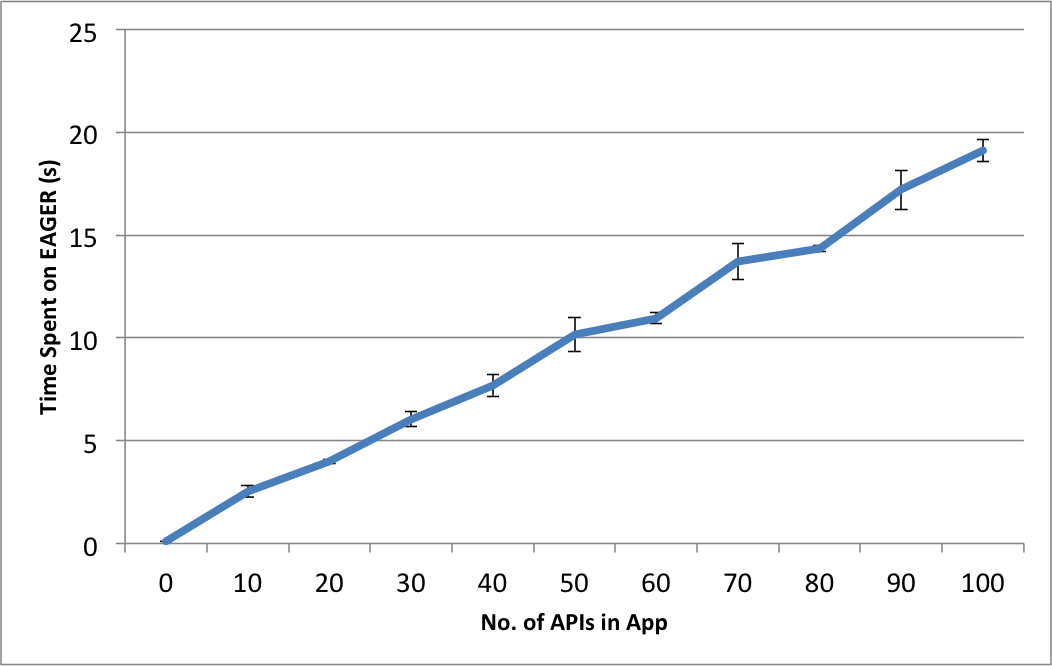
\includegraphics[scale=0.45]{overhead_by_apis}
\vspace{-0.01in}
\caption{EAGER Overhead vs. Number of APIs Exported by the Application}
\label{fig:overhead_by_apis}
%\vspace{-0.1in}
\end{figure}

At present we expect most applications deployed in cloud to have a small to 
moderate number of APIs ($10$ or fewer).  With this API density EAGER's current 
scaling is adequate.  Even in the
unlikely case that a single application exports as many as $100$ APIs,
the total time for EAGER is under $20$ seconds.

Next, we analyze EAGER overhead as the number of dependencies declared in
an application grows. For this experiment, we first populate the EAGER
Metadata Manager with metadata for $100$ randomly generated APIs. Then we
deploy an application on EAGER which exports a single API and declares
dependencies on the fictitious 
APIs that are already stored in the Metadata Manager. We
vary the number of declared dependencies and observe the EAGER overhead.

\begin{figure}
\centering
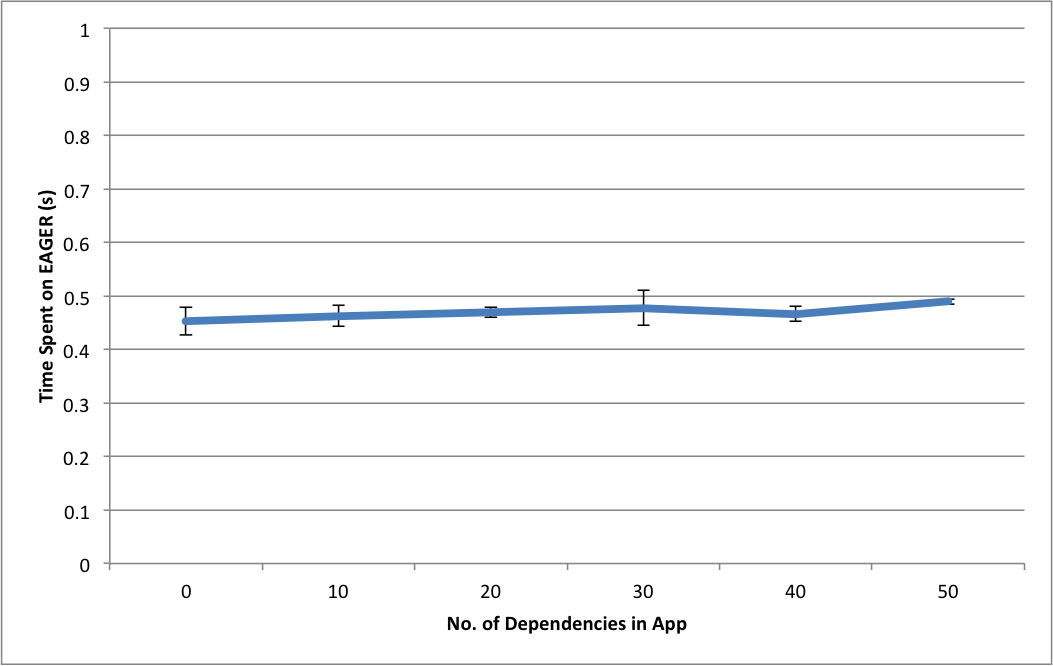
\includegraphics[scale=0.45]{overhead_by_deps}
\vspace{-0.01in}
\caption{EAGER Overhead vs. Number of Dependencies Declared in the Application}
\label{fig:overhead_by_deps}
%\vspace{-0.1in}
\end{figure}

Figure~\ref{fig:overhead_by_deps} shows the results of these experiments. 
EAGER overhead does not appear to be significantly
influenced by the number of dependencies declared in an application. 
In this case, the EAGER implementation processes
all dependency-related information via batch operations. 
As a result, the number of web service calls and database queries that originate 
due to varying number of dependencies is fairly constant. 

\subsection{Impact of Number of Policies}

So far we have conducted all our experiments without any active governance 
policies in the system. In this section, we report how EAGER overhead
is impacted by the number of policies.

The overhead of policy validation is largely dependent on the actual policy
content (Python code). Since users may include any Python code 
(as long as it falls in the accepted subset) in a policy file, evaluating a
given policy can take an arbitrary amount of time.  Therefore, in this
experiment, our goal is to evaluate the overhead incurred by simply having
many policy files to execute. We keep the content of the policies small and
trivial. We create a policy file that runs following assertions:
\begin{enumerate} 
\item Application name must start with an upper case letter
\item Application must be owned by a specific user 
\item All API names must start with upper case letters 
\end{enumerate} We create many copies of this
initial policy file to vary the number of policies deployed. Then we evaluate
the overhead of policy validation on two of our sample applications
(guestbook-py and simple-jaxrs-app). 

\begin{figure}
\centering
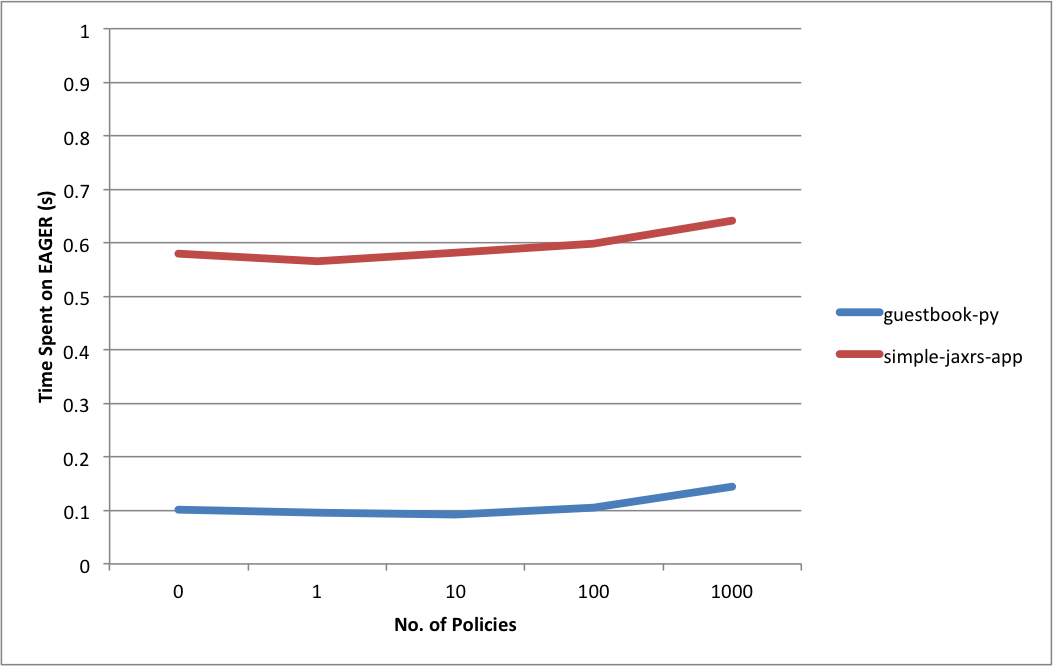
\includegraphics[scale=0.45]{overhead_by_policies}
\vspace{-0.01in}
\caption{EAGER Overhead vs. Number of Policies}
\label{fig:overhead_by_policies}
%\vspace{-0.1in}
\end{figure}

Figure~\ref{fig:overhead_by_policies} shows how the number of active policies
impact EAGER overhead. Interestingly, even large numbers of policies 
do not impact EAGER overhead significantly. It is only when the active
policy count approaches $1000$ that we can see a small increase in the
overhead. Even then, the increase in deployment time is under $0.1$ seconds. 

This result due to the fact that EAGER loads policy content into memory at system
startup (or when a new policy is deployed), and executes them from memory each
time an application is deployed. Since policy files are typically small (at
most a few kilobytes), this is a viable option. The overhead of validating the
simple-jaxrs-app is higher than that of the guestbook-py because,
simple-jaxrs-app exports web APIs. This means the third assertion in the
policy set is executed for this app and not for guestbook-py. 

Out results indicate that EAGER scales well to hundreds of policies. That is,
there is no significant overhead associated with simply having a large number
of policy files. However, as mentioned earlier, the content of a policy may
influence the overhead of policy validation and will be specific to the policy and 
application EAGER analyzes.
 
\subsection{Scalability}
Next, we evaluate how EAGER scales when a large number of APIs are deployed 
in the cloud. In this experiment, we populate the EAGER
Metadata Manager with a varying number of APIs. We then attempt to deploy various sample 
applications. We also create random dependencies among the APIs recorded in the 
Metadata Manager to make the experimental setting more realistic.

\begin{figure}
\centering
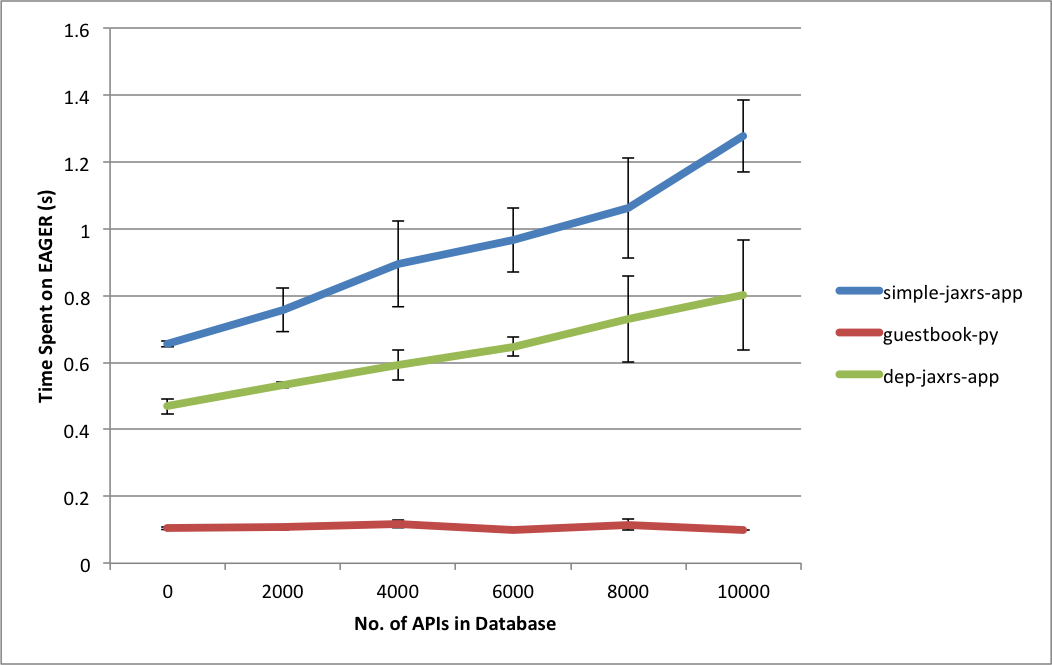
\includegraphics[scale=0.45]{scalability}
\vspace{-0.01in}
\caption{EAGER Overhead vs. Number of APIs in Metadata Manager}
\label{fig:scalability}
%\vspace{-0.1in}
\end{figure}

Figure~\ref{fig:scalability} shows that the deployment overhead of the 
guestbook-py application is not impacted by the growth of metadata
in the cloud. Recall that guestbook-py does not export any APIs nor does it 
declare any dependencies. Therefore the deployment process of
the guestbook-py application has minimal interactions with the 
Metadata Manager. Based on this result we conclude that applications that
do not export web APIs are not significantly affected by the accumulation 
of metadata in EAGER.

Both simple-jaxrs-app and dep-jaxrs-app are
affected by the volume of data stored in Metadata Manager. Since these applications 
export web APIs that must be recorded and validated by the Metadata Manager, 
the growth of metadata has an increasingly higher impact on them. The degradation 
of performance is due to the slow query performance of the RDBMS engine (MySQL) 
as the database size grows. The simple-jaxrs-app
is affected more by this performance drop, because it exports two APIs compared to the single API exported 
by dep-jaxrs-app. However, the growth
in overhead is linear to the number of APIs deployed in the cloud. Also,
even after deploying $10000$ APIs, the overhead on simple-jaxrs-app is only been increased by 
about $0.5$ seconds.

Another interesting characteristic in Figure~\ref{fig:scalability} is the
increase in overhead variance as the number of APIs in the cloud
grows.  We believe this is due to the increasing variability of database query
performance and the data transfer performance as the size of the database
increases.

In summary, the current EAGER prototype scales well to $1000$'s of APIs.
If further scalability is required, there are opportunities to enable it
via parallelization and database query optimization.

\subsection{Experimental Results with a Real-World Dataset}

Finally, we explore how EAGER operates with a real-world dataset with API
metadata and dependency information. For this, we crawl the ProgrammableWeb
registry and extract metadata regarding all registered APIs and mashups.
At the time of the experiment, we collected $11095$ APIs and $7227$ 
mashups (each mashups depends on one or more APIs).

We populated the EAGER Metadata Manager with these APIs and
registered each of the mashups as APIs in EAGER. We then used the
mashup-API dependency information to register dependencies among the APIs in 
EAGER. This resulted in a total dependency graph of $18322$ APIs 
with $33615$ dependencies.  We the deploy a subset of our applications
and measure EAGER overhead.

\begin{figure}
\centering
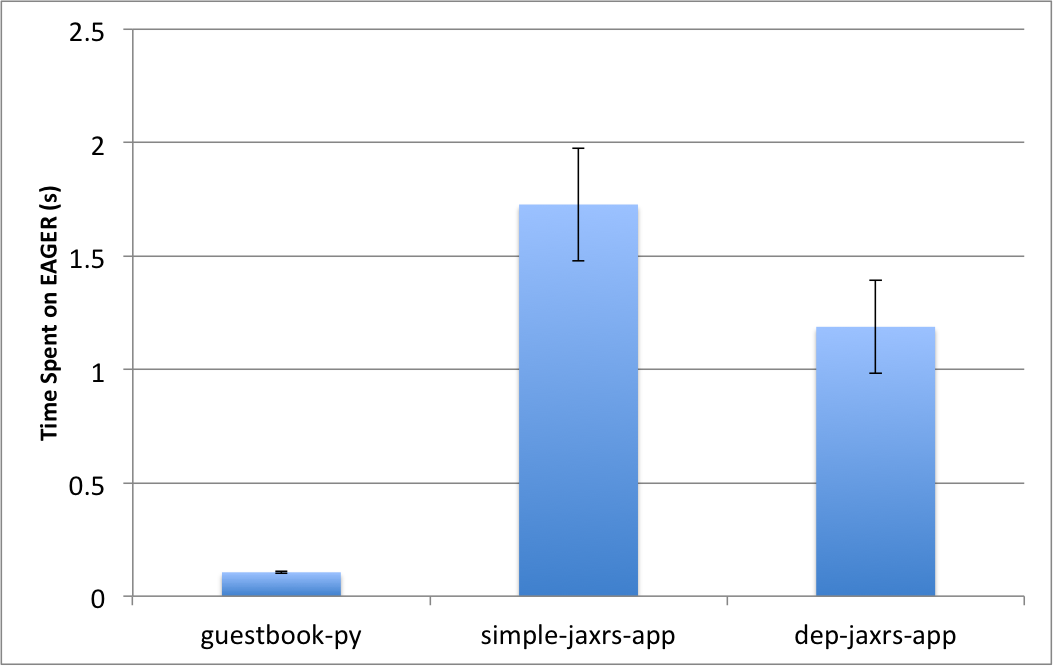
\includegraphics[scale=0.45]{pweb_sample_overhead}
\vspace{-0.01in}
\caption{EAGER Overhead When Deploying on ProgrammableWeb Dataset}
\label{fig:pweb_sample_overhead}
%\vspace{-0.1in}
\end{figure}

Figure~\ref{fig:pweb_sample_overhead} shows the results for three applications. The guestbook-py app
(without any web APIs) is not significantly impacted by the large dependency database. 
Applications that export web APIs show a slightly higher deployment overhead. 
The highest overhead observed is under 2 seconds, which is a small percentage
of total application deployment time. 

The applications in this experiment do not declare dependencies on any of the APIs 
in the ProgrammableWeb dataset. The dep-jaxrs-app does declare a dependency, 
but that is on an API exported by 
simple-jaxrs-app. To see how the deployment time is impacted
when applications become dependent on other APIs registered in EAGER, we
deploy a test application that declares random fictitious dependencies on APIs
from the ProgrammableWeb corpus registered in EAGER.  We consider 
$10$, $20$, and $50$ declared dependencies and deploy each
the application three times.
We present the results in Figure~\ref{fig:pweb_random_overhead}.
For the ``random'' datasets, we
run a deployment script that randomly modifies the 
declared dependencies at each redeployment. For the 
``fixed'' datasets the declared dependencies remains the same across
redeployments.

\begin{figure}
\centering
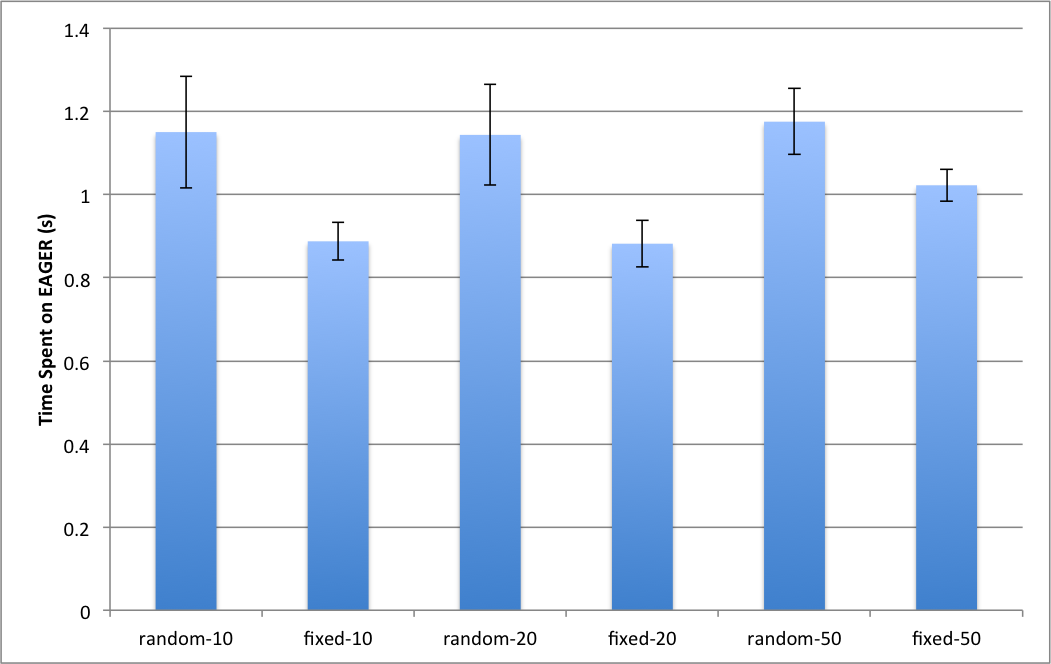
\includegraphics[scale=0.45]{pweb_random_overhead}
\vspace{-0.01in}
\caption{EAGER Overhead When Deploying on ProgrammableWeb Dataset with
Dependencies. The suffix value indicates the number of dependencies;
the prefix indicates if these dependencies are randomized (or not) upon
redeployment.  We present the average overhead in seconds across three redeployments.
\label{fig:pweb_random_overhead}
}
\end{figure}


Interestingly, dependency count does not have a significant impact on 
the overhead.  The largest overhead observed is under 1.2 seconds.
In addition, when the dependency declaration is fixed, the overhead is slightly smaller. 
This is because our prototype caches the edges of its internally generated dependency tree, 
which expedites redeployments.

In summary, EAGER adds a very small overhead to the application deployment
process, and 
this overhead increases linearly with the number of APIs exported by the applications
and the number of APIs deployed in the cloud. 
Interestingly, the number of deployed policies and declared dependencies
have little impact on the EAGER governance overhead. 
Finally, our results indicate that EAGER scales 
well to $1000$'s of APIs and adds no more than $2$ seconds with over
$18,000$ ``real-world'' deployed APIs in its database.
